\documentclass[12pt]{beamer}
\usepackage{../Estilos/BeamerMAF}
\usepackage[absolute, overlay]{textpos}
\usepackage{../Estilos/ColoresLatex}
%Sección para el tema de beamer, con el theme, usercolortheme y sección de footers
\usetheme{Antibes}
\usecolortheme{beaver}
%\useoutertheme{default}
\setbeamercovered{invisible}
% or whatever (possibly just delete it)
\setbeamertemplate{section in toc}[sections numbered]
\setbeamertemplate{subsection in toc}[subsections numbered]
\setbeamertemplate{subsection in toc}{\leavevmode\leftskip=3.2em\rlap{\hskip-2em\inserttocsectionnumber.\inserttocsubsectionnumber}\inserttocsubsection\par}
\setbeamercolor{section in toc}{fg=blue}
\setbeamercolor{subsection in toc}{fg=blue}
%\setbeamercolor{frametitle}{fg=blue}
\setbeamertemplate{caption}[numbered]

\setbeamertemplate{footline}
\beamertemplatenavigationsymbolsempty
\setbeamertemplate{headline}{}


\makeatletter
\setbeamercolor{secºtion in foot}{bg=gray!30, fg=black!90!orange}
\setbeamercolor{subsection in foot}{bg=blue!30!yellow, fg=red}
\setbeamercolor{date in foot}{bg=black, fg=white}
\setbeamertemplate{footline}
{
  \leavevmode%
  \hbox{%
  \begin{beamercolorbox}[wd=.333333\paperwidth,ht=2.25ex,dp=1ex,center]{section in foot}%
    \usebeamerfont{section in foot} \insertsection
  \end{beamercolorbox}%
  \begin{beamercolorbox}[wd=.333333\paperwidth,ht=2.25ex,dp=1ex,center]{subsection in foot}%
    \usebeamerfont{subsection in foot}  \insertsubsection
  \end{beamercolorbox}%
  \begin{beamercolorbox}[wd=.333333\paperwidth,ht=2.25ex,dp=1ex,right]{date in head/foot}%
    \usebeamerfont{date in head/foot} \insertshortdate{} \hspace*{2em}
    \insertframenumber{} / \inserttotalframenumber \hspace*{2ex} 
  \end{beamercolorbox}}%
  \vskip0pt%
}







\setbeamercolor{section in foot}{bg=amethyst, fg=white}
\setbeamercolor{subsection in foot}{bg=almond, fg=black}

\makeatletter
\setbeamertemplate{footline}
{
\leavevmode%
\hbox{%
\begin{beamercolorbox}[wd=.333333\paperwidth,ht=2.25ex,dp=1ex,center]{section in foot}%
  \usebeamerfont{section in foot} \insertsection
\end{beamercolorbox}%
\begin{beamercolorbox}[wd=.333333\paperwidth,ht=2.25ex,dp=1ex,center]{subsection in foot}%
  \usebeamerfont{subsection in foot}  \insertsubsection
\end{beamercolorbox}%
\begin{beamercolorbox}[wd=.333333\paperwidth,ht=2.25ex,dp=1ex,right]{date in head/foot}%
  \usebeamerfont{date in head/foot} \insertshortdate{} \hspace*{1.5em}
  \insertframenumber{} / \inserttotalframenumber \hspace*{2ex} 
\end{beamercolorbox}}%
\vskip0pt%
}
\makeatother
\usefonttheme{serif}
\setbeamercolor{frametitle}{bg=champagne}
\resetcounteronoverlays{saveenumi}

\date{31 de mayo de 2022}

\title{\large{Transformada de Fourier - Ejercicios}}
\subtitle{Matemáticas Avanzadas de la Física}
\author{M. en C. Gustavo Contreras Mayén}

\begin{document}
\maketitle
\fontsize{14}{14}\selectfont
\spanishdecimal{.}

\section*{Contenido}
\frame[allowframebreaks]{\frametitle{Temas a revisar} \tableofcontents[currentsection, hideallsubsections]}

\section{La Transformada de Fourier}
\frame[allowframebreaks]{\frametitle{Contenido}\tableofcontents[currentsection, hideothersubsections]}
\subsection{Ejercicios}

\subsection*{Ejercicio 1}
%Ref. Patra (2018) . Example 1.4
\begin{frame}
\frametitle{Enunciado}
Calcula la función cuya Transformada coseno de Fourier es:
\pause
\begin{align*}
\sqrt{\dfrac{2}{\pi}} \, \dfrac{\sin a \, \xi}{\xi}
\end{align*}
\end{frame}
\begin{frame}
\frametitle{Graficando la Transformada coseno de Fourier}
\begin{figure}
  \centering
  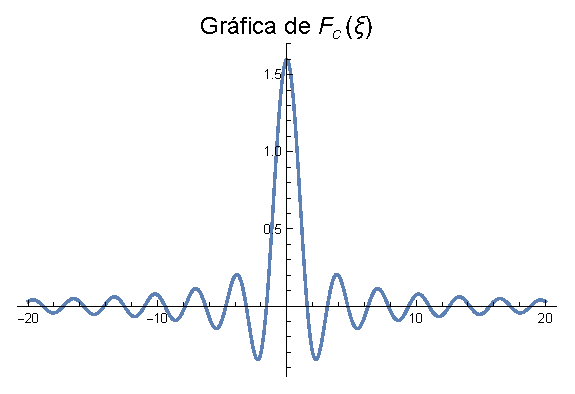
\includegraphics[scale=1]{Imagenes/Plot_Fourier_Ejercicios_01_sinc_x.eps}
\end{figure}
\end{frame}
\begin{frame}
\frametitle{Solución}
Sabemos que la transformada coseno de Fourier es:
\pause
\begin{align*}
F_{c} \big[ f (x); x \to \xi \big] = \sqrt{\dfrac{2}{\pi}} \, \dfrac{\sin a \, \xi}{\xi}
\end{align*}
\end{frame}
\begin{frame}
\frametitle{Usando la TCIF}
La Transformada Coseno Inversa de Fourier (TCIF), está dada por la expresión:
\pause
\begin{align*}
f (x) = \sqrt{\dfrac{2}{\pi}} \scaleint{6ex}_{\bs 0}^{\infty} F_{c} (\xi) \, \cos \xi \, x \dd{\xi}
\end{align*}
\end{frame}
\begin{frame}
\frametitle{Usando la TCIF}
Entonces por la definición anterior:
\pause
\begin{align*}
f (x) = \dfrac{2}{\pi} \scaleint{6ex}_{\bs 0}^{\infty} \dfrac{\sin a \, \xi}{\xi} \, \cos \xi \, x \dd{\xi}
\end{align*}
\pause
Ahora tendremos que hacer uso extensivo de nuestras habilidades en el álgebra e integración para resolver la expresión.
\end{frame}
\begin{frame}
\frametitle{Identidad trigonométrica}
Usamos una identidad trigonométrica del producto:
\pause
\begin{align*}
\sin x \, \cos y = \dfrac{\sin (x + y) + \sin (x - y)}{2}
\end{align*}
\pause
Tenemos entonces que:
\begin{eqnarray*}
\begin{aligned}
\sin a \, \xi \, \cos \xi \, x &= \dfrac{\sin \big[ a \xi + \xi x \big] + \sin \big[ a \xi - \xi x \big]}{2} = \\[0.5em] \pause
&= \dfrac{\sin \big[ \xi (a + x) \big] + \sin \big[ \xi (a - x) \big]}{2}
\end{aligned}
\end{eqnarray*}
\end{frame}
\begin{frame}
\frametitle{Ajuste en la expresión}
Ahora la TCIF es:
\pause
\begin{eqnarray*}
\begin{aligned}
f (x) &= \dfrac{1}{\pi} \scaleint{6ex}_{\bs 0}^{\infty} \dfrac{1}{\xi} \, \sin \big[ \xi (a + x) \big] + \sin \big[ \xi (a - x) \big] \dd{\xi} = \\[0.5em] \pause
&= \dfrac{1}{\pi} \bigg[ \scaleint{6ex}_{\bs 0}^{\infty} \dfrac{\sin \big[ \xi (a + x) \big]}{\xi} \dd{x} + \\[0.5em] 
&+ \scaleint{6ex}_{\bs 0}^{\infty} \dfrac{\sin \big[ \xi (a - x) \big]}{\xi} \dd{x} \bigg] =
\end{aligned}
\end{eqnarray*}
\end{frame}
\begin{frame}
\frametitle{Integral especial}
\begin{minipage}{0.5\linewidth}
En ambas integrales tenemos una integral particular: \pause la integral del seno cardinal:
\pause
\begin{align*}
\scaleint{6ex}_{\bs -\infty}^{\infty} \dfrac{\sin x}{x} \dd{x}
\end{align*}
\end{minipage}
\pause
\begin{minipage}{0.4\linewidth}
\begin{figure}
  \centering
  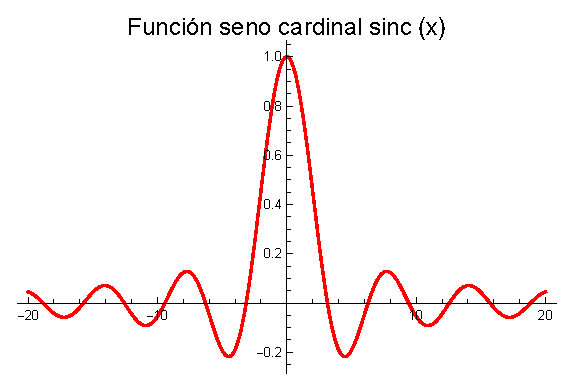
\includegraphics[scale=0.6]{Imagenes/Plot_Fourier_Ejercicios_02_sinc_x.eps}
\end{figure}
\end{minipage}
\end{frame}
\begin{frame}
\frametitle{Resultado del Cálculo II}
Sabemos del curso de Cálculo II, que el valor de la integral del seno cardinal es:
\pause
\begin{eqnarray*}
\scaleint{6ex}_{\bs -\infty}^{\infty} \dfrac{\sin x}{x} \dd{x} = \pause \pi
\end{eqnarray*}
\pause
Por tanto:
\pause
\begin{eqnarray*}
\scaleint{6ex}_{\bs 0}^{\infty} \dfrac{\sin x}{x} \dd{x} = \pause \dfrac{\pi}{2}
\end{eqnarray*}
\end{frame}
\begin{frame}
\frametitle{Revisando el integrando}
Como ya sabemos el valor de la integral seno cardinal, tenemos que revisar previamente el argumento de la función seno, \pause es decir, para qué valores no se anula.
\end{frame}
\begin{frame}
\frametitle{Revisando el integrando}
Se tiene entonces que:
\begin{eqnarray*}
\begin{aligned}
\sin \big[ \xi (a + x) \big] \pause \hspace{0.2cm} \Rightarrow \hspace{0.2cm} \mbox{si } x < a \pause \mbox{ no se anula} \\[0.5em] \pause
\sin \big[ \xi (a - x) \big] \pause \hspace{0.2cm} \Rightarrow \hspace{0.2cm} \mbox{si } x > a \pause \mbox{ no se anula}
\end{aligned}
\end{eqnarray*}
\end{frame}
\begin{frame}
\frametitle{El valor de la integral}
Entonces tenemos lo siguiente:
\begin{eqnarray*}
\begin{aligned}
f (x) = \begin{cases}
\dfrac{1}{\pi} \bigg[ \dfrac{\pi}{2} + \dfrac{\pi}{2} \bigg] & \mbox{si } x < a \\[1em]
\dfrac{1}{\pi} \bigg[ \dfrac{\pi}{2} - \dfrac{\pi}{2} \bigg] & \mbox{si } x > a
\end{cases}
\end{aligned}
\end{eqnarray*}
\end{frame}
\begin{frame}
\frametitle{La función buscada}
Entonces la función $f (x)$ pedida en el enunciado es:
\begin{align*}
f (x) = \begin{cases}
1 & \mbox{si } x < a \\[1em]
0 & \mbox{si } x > a
\end{cases}
\end{align*}
\end{frame}
\begin{frame}
\frametitle{Gráfica de la función $f (x)$}
\begin{figure}
  \centering
  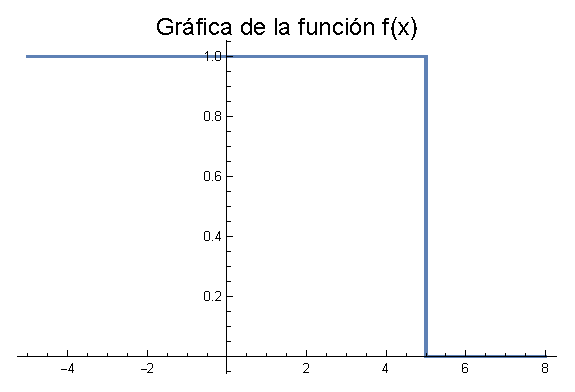
\includegraphics[scale=1]{Imagenes/Plot_Fourier_Ejercicios_03_sinc_x.eps}
\end{figure}
\end{frame}

\subsection*{Ejercicio 2}

\begin{frame}
\frametitle{Ejercicio 2 - Enunciado}
Calcula la Transformada de Fourier de:
\pause
\begin{align*}
f (x) = \begin{cases}
1 -x^{2}, & \abs{x} \leq 1 \\
0 & \abs{x} > 1
\end{cases}
\end{align*}
\pause
y con ello evaluar:
\pause
\begin{align*}
\scaleint{6ex}_{\bs 0}^{\infty} \dfrac{x \, \cos x - \sin x}{x^{3}} \, \cos \bigg( \dfrac{x}{2} \bigg) \dd{x}
\end{align*}
\end{frame}
\begin{frame}
\frametitle{Gráfica de $f(x)$}
\begin{figure}
  \centering
  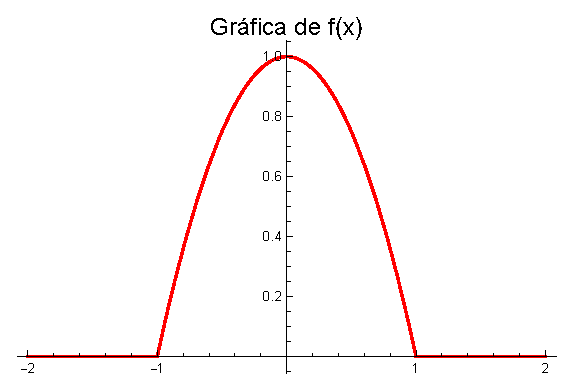
\includegraphics[scale=1]{Imagenes/Plot_Fourier_Ejercicio_02_01.eps}
\end{figure}
\end{frame}
\end{document}